\section{线性价值函数逼近求解投影 Bellman 方程}
\label{sec:16-Control-and-Reinforcement-Learning/02-Reinforcement-Learning/05}

冷库控制器的状态是二十四个传感器读数拼成的连续向量。表格法在这里第一步就走不下去：状态不可枚举，存不下；就算存得下，相邻零点几度的两个状态也会被当成毫不相干的格子，一个状态学到的东西传不到隔壁。

于是你把值函数换成

\[
\widehat V(s;w)=\phi(s)^{\trans}w,
\]

\(\phi(s)\in\R^m\) 是特征向量。one-hot 特征让每个状态只激活一个坐标，退化回表格；一般特征让许多状态共享参数，这既带来泛化，也意味着一次更新会顺手改动大量没访问过的状态。TD 照跑，参数照收敛，但收敛到的那个东西已经不是上一节的 \(V^\pi\)，甚至不是 \(V^\pi\) 在特征空间里的最佳近似。这一节要说清它到底是什么。

\subsection{换成特征之后，``最准''要先说清在哪些状态上准}

固定策略 \(\pi\)。假设真实价值 \(V^\pi\) 已知，最自然的目标是加权平方误差

\[
J_{\mathrm{VE}}(w)
=\frac12\sum_s d(s)\bigl(V^\pi(s)-\phi(s)^{\trans}w\bigr)^2 .
\]

权重 \(d\) 不是可以略过的技术细节。表格法里根本没有这个东西——每个状态各管各的，谈不上取舍。参数一共享，特征装不下的那部分误差就必须分配到某处，\(d\) 决定分配方案。均匀权重平等对待所有状态；策略的长期访问分布 \(d^\pi\) 偏袒常见状态；折扣占用分布还会带上初始分布的影响。谁是``最佳近似''，取决于你用哪个 \(d\) 提问。

把 \(\Phi\) 的第 \(s\) 行取作 \(\phi(s)^{\trans}\)，记 \(D=\diag(d)\)。任一状态值向量 \(v\) 在 \(D\)-加权内积下往 \(\operatorname{col}(\Phi)\) 的正交投影是

\[
\Pi_Dv=\Phi(\Phi^{\trans}D\Phi)^{-1}\Phi^{\trans}Dv,
\]

前提是 \(\Phi^{\trans}D\Phi\) 可逆。这个式子与\hyperref[sec:03-Linear-Algebra/03-Orthogonality/02]{``投影与最近点：从一条直线走向一般子空间''}里的投影矩阵是同一个东西，只是内积换成了带权的那一个。特征若在 \(d\) 覆盖到的状态上共线，参数不可识别，要么删冗余特征，要么给线性系统加正则。

\subsection{TD 的更新是半梯度，不是对某个损失的普通梯度}

真实的 \(V^\pi(S_t)\) 不可观察，只能找代理。完整回报满足 \(\E_\pi[G_t\given S_t=s]=V^\pi(s)\)，所以

\[
w_{t+1}=w_t+\alpha_t\bigl(G_t-\widehat V(S_t;w_t)\bigr)\phi(S_t)
\]

确实是回归目标的随机梯度步，没有自举，要付出的是等待与方差。一步 TD 换成

\[
Y_t=R_{t+1}+\gamma\widehat V(S_{t+1};w_t),
\qquad
\delta_t=Y_t-\widehat V(S_t;w_t),
\qquad
w_{t+1}=w_t+\alpha_t\delta_t\phi(S_t).
\]

外形一模一样，但求导时把 \(Y_t\) 当成了常数——目标里的 \(\widehat V(S_{t+1};w_t)\) 明明也依赖 \(w_t\)，那条链没有被求导。这叫半梯度。若对单样本的平方 TD 误差完整求导，方向里会多出 \(-\gamma\phi(S_{t+1})\) 一项，得到的是 residual-gradient 类方法，行为与 TD 不同。更新式长得像监督学习，不等于它在对某个固定损失做 SGD；接下来要问的正是：既然它不是任何显式损失的梯度，那它收敛到哪儿？

\subsection{期望更新暴露了 TD 实际在解的方程}

设 \(P_\pi\) 是策略诱导的转移矩阵，\(r_\pi\) 是期望即时奖励，样本状态取自 \(d^\pi\)，\(D=\diag(d^\pi)\)。把 TD 更新方向取期望并整理，

\[
\E[\delta_t\phi(S_t)]=b-Aw,
\qquad
A=\Phi^{\trans}D(I-\gamma P_\pi)\Phi,
\qquad
b=\Phi^{\trans}Dr_\pi .
\]

迭代若收敛，极限 \(w_*\) 必满足 \(Aw_*=b\)。把策略 Bellman 算子记为 \(T_\pi v=r_\pi+\gamma P_\pi v\)，这个线性方程可以改写成

\[
\Phi w_*=\Pi_D T_\pi(\Phi w_*).
\]

这就是投影 Bellman 方程。它与上一节那个不动点方程差了一个 \(\Pi_D\)，而这一个符号改变了整件事的性质：\(T_\pi\) 作用在一个可表示的向量上，结果一般会离开 \(\operatorname{col}(\Phi)\)；要求 \(\Phi w=T_\pi(\Phi w)\) 通常无解，因为等号右边压根不在左边所在的空间里。TD 求的不是 Bellman 算子的不动点，而是``先做一次 Bellman 更新，再投影回可表示空间''这个复合算子的不动点。

\begin{center}
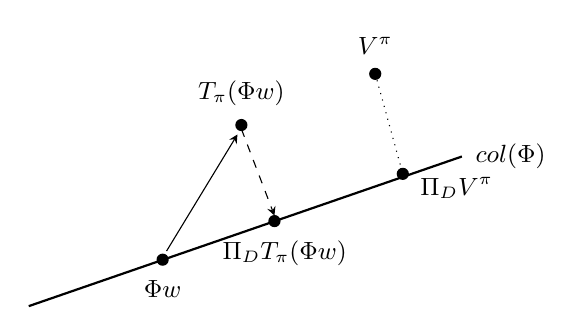
\begin{tikzpicture}[>=stealth, scale=1.0]
% 可表示空间
\draw[thick] (0.3,0.6) -- (5.8,2.50);
\node[anchor=west] at (5.85,2.50) {\small \(\operatorname{col}(\Phi)\)};
% Phi w
\fill (2.0,1.19) circle (2.2pt);
\node[anchor=north] at (2.0,1.05) {\small \(\Phi w\)};
% T_pi (Phi w)
\fill (3.0,2.90) circle (2.2pt);
\node[anchor=south] at (3.0,3.02) {\small \(T_\pi(\Phi w)\)};
\draw[->] (2.05,1.30) -- (2.95,2.78);
% 投影回来
\draw[dashed,->] (3.0,2.85) -- (3.42,1.75);
\fill (3.42,1.68) circle (2.2pt);
\node[anchor=north] at (3.55,1.55) {\small \(\Pi_DT_\pi(\Phi w)\)};
% V^pi 与其最佳近似
\fill (4.7,3.55) circle (2.2pt);
\node[anchor=south] at (4.7,3.67) {\small \(V^\pi\)};
\draw[dotted] (4.7,3.55) -- (5.05,2.28);
\fill (5.05,2.28) circle (2.2pt);
\node[anchor=west] at (5.15,2.10) {\small \(\Pi_DV^\pi\)};
\end{tikzpicture}
\end{center}

\emph{Bellman 更新把点抬离可表示空间，投影再把它压回来；TD 找的是这一抬一压的不动点，而它一般不等于 \(V^\pi\) 的最佳近似。}

图里最该盯住的是右上角那两个点没有被任何箭头连到左边的循环上。\(\Pi_DV^\pi\) 是你如果知道真值会选的那个最佳近似，而 TD 的不动点是那条抬压循环的归宿，两者不重合。差距是可以估计的：在 on-policy 权重下，

\[
\norm{\Phi w_*-V^\pi}_D
\le
\frac{1}{1-\gamma}\norm{\Pi_DV^\pi-V^\pi}_D .
\]

不可表示的那部分误差被放大了 \(1/(1-\gamma)\) 倍才交到你手上。\(\gamma=0.99\) 时这个系数是 \(100\)——特征稍差一点，最终价值误差就可能大得离谱，而参数本身收敛得干干净净。

还有一条边界要划清。半梯度 TD 是对 \(b-Aw=0\) 的随机逼近，不能笼统说成``对投影 Bellman 误差做随机梯度下降''。若定义

\[
J_{\mathrm{PBE}}(w)=\norm{\Phi w-\Pi_DT_\pi(\Phi w)}_D^2,
\]

它的零点与投影方程一致，但它的真实梯度一般不是 \(-\E[\delta_t\phi(S_t)]\)。Gradient-TD 类方法存在的理由，就是去构造一个能由样本估计的、真正的梯度目标。

\subsection{投影既是稳定的来源，也是不稳定的来源}

on-policy 情形下这套东西为什么还稳得住？骨架是两个非扩张性拼起来。\(T_\pi\) 在 \(\norm{\cdot}_D\) 下是模 \(\gamma\) 的压缩，这依赖一个关键事实：\(d^\pi\) 是 \(P_\pi\) 的平稳分布，所以 \(P_\pi\) 在这个加权范数下不放大长度。而正交投影 \(\Pi_D\) 在\emph{同一个} \(D\)-范数下非扩张，这是投影的基本性质。两者复合，压缩系数仍是 \(\gamma<1\)，Banach 不动点定理照旧适用，唯一解存在，TD 作为它的随机逼近在遍历性、有界性、Robbins--Monro 步长下收敛。

条件对账里最脆的一根是``同一个范数''。压缩性属于 \(T_\pi\) 在 \(\norm{\cdot}_{d^\pi}\) 下，非扩张性属于 \(\Pi_D\) 在 \(\norm{\cdot}_D\) 下，只有当 \(D\) 就是 \(d^\pi\)——也就是数据确实由待评价策略产生——两者才谈得上相乘。数据换成别的策略采的，\(D\) 变成另一个分布，\(\Pi_D\) 仍在它自己的范数下非扩张，却可能在 \(T_\pi\) 压缩的那个范数下把误差放大。复合算子的压缩性就此失去依据，它甚至可能是扩张的，参数发散而不是收敛。

这条裂缝值得记牢：\hyperref[sec:03-Linear-Algebra/03-Orthogonality/01]{``正交与正交补：把空间分成互不干扰的方向''}里的投影非扩张性，是相对于定义它的那个内积说的。换了权重就是换了内积，两个不同内积下的``不放大''不能相乘。下一节的 Deadly Triad——函数逼近、自举、离策略数据三者同时出现——正是这条裂缝被撑开之后的样子，而撑开它的第一道口子就在这里的 \(\Pi_D\)。

顺带说一句 one-hot 的情形：此时 \(\Phi=I\)，投影是恒等映射，裂缝不存在，极限就是精确的 \(V^\pi\)。表格法的稳定不是运气，是因为它根本没有投影这一步。

收敛也不等于误差小。真实价值曲面若不在 \(\operatorname{col}(\Phi)\) 中，表示误差永远存在；\(d^\pi\) 很小的状态即使错得离谱也几乎不影响目标；而部署之后策略一变，重要的状态跟着变，原先``拟合良好''的那个加权范数就不再是你关心的度量了。

\subsection{直接解线性系统，难处挪到统计与数值上}

既然要解的是 \(Aw=b\)，也可以不迭代，直接从样本估

\[
\widehat A=\sum_t\phi(S_t)\bigl(\phi(S_t)-\gamma\phi(S_{t+1})\bigr)^{\trans},
\qquad
\widehat b=\sum_tR_{t+1}\phi(S_t),
\]

再解 \(\widehat Aw=\widehat b\)。这就是 LSTD，它比逐步 TD 更充分地用掉每个样本，为此要维护一个 \(m\times m\) 矩阵，并承担它的条件数。实现时应当解线性系统而不是显式求逆，理由与\hyperref[sec:08-Numerical-Analysis/07-Numerical-Methods-for-ML/03]{``需要的是解，而不是逆矩阵''}里说的完全一致。样本相关、覆盖不足或特征近共线都会让 \(\widehat A\) 病态，此时正则化不是可选项。

诊断线性价值逼近时，三件事要分开看：参数更新是否稳定，投影 Bellman 残差是否在变小，以及在你真正关心的状态分布上价值误差是否可接受。三者互不蕴含——参数可以稳稳收敛而误差很大，残差可以很小而策略很差。下一节把 on-policy 这个条件拿掉，看那道裂缝被撑开之后会发生什么。
